\documentclass[12pt,letterpaper]{article}

% ---------- Idioma y codificación ----------
\usepackage[spanish,es-noshorthands]{babel}
\usepackage[utf8]{inputenc}
\usepackage[T1]{fontenc}
\usepackage{csquotes}

% ---------- Estructura y layout ----------
\usepackage{tabularx}
\usepackage{float}
\usepackage{scrhack}
\usepackage[margin=2.5cm]{geometry}

% ---------- Tipografía ----------
\usepackage{newtxtext}
\usepackage{newtxmath}
\usepackage{setspace}
\onehalfspacing

% ---------- Imágenes y tablas ----------
\usepackage{graphicx}
\usepackage{booktabs}
\usepackage{xcolor}
\usepackage{enumitem}

% ---------- Placeholder visual ----------
\newcommand{\relleno}{\textcolor{red}{\itshape [completar]}}

%\title{\vspace{-1.5cm}Variable estadística: Lenguaje de programación favorito}
%\author{Facultad de Ingeniería de Producción y Servicios (FIPS)}
%\date{}

\begin{document}
%\maketitle
%\thispagestyle{empty}

% =========================================================
% ================ FICHA TÉCNICA DE LA VARIABLE ==========
% =========================================================
\section*{Ficha técnica}

\begin{tabularx}{\textwidth}{@{}l X@{}}
\textbf{Variable estadística $X$:} & Lenguaje de programación favorito (FIPS) \\[4pt]
\textbf{Población:} & Estudiantes de 2do año de Ingeniería de Sistemas \\[4pt]
\textbf{Muestra:} & 22 estudiantes de EMAT, grupo B \\[4pt]
\textbf{Unidad de observación:} & Un estudiante individual \\[4pt]
\textbf{Fuente:} & Recolección de datos mediante formulario de Google Forms \\[4pt]
\textbf{Tipo de dato estadístico:} & Cualitativo nominal \\
\end{tabularx}

\vspace{1cm}

% =========================================================
% ============ TABLA DE DISTRIBUCIÓN DE FRECUENCIAS ======
% =========================================================
\section*{Tabla de distribución de frecuencias}

\begin{table}[H]
    \centering
    \caption{Lenguajes de programación favoritos de los estudiantes de EMAT B (FIPS)}
    \label{tab:lenguajes-favoritos}
    \begin{tabular}{@{}lccc@{}}
        \toprule
        \textbf{Lenguaje ($x_i$)} & \textbf{Frecuencia absoluta ($f_i$)} & \textbf{Frecuencia relativa ($h_i$)} & \textbf{Porcentaje (\%)} \\
        \midrule
        Java        & 14 & 0.6364 & 63.64\% \\
        Python      & 1 & 0.0455 & 4.55\% \\
        JavaScript  & 1 & 0.0455 & 4.55\% \\
        C++         & 5 & 0.2273 & 22.73\% \\
        Otro        & 1 & 0.0455 & 4.55\% \\
        \midrule
        \textbf{Total} & 22 & 1.0000 & 100\% \\
        \bottomrule
    \end{tabular}
\end{table}

\noindent\textit{Nota: al ser una variable cualitativa nominal, no corresponde calcular frecuencias acumuladas, ya que las categorías no tienen un orden intrínseco.}

% =========================================================
% ==================== DIAGRAMAS ==========================
% =========================================================
\section*{Representación gráfica}

\begin{figure}[H]
    \centering
    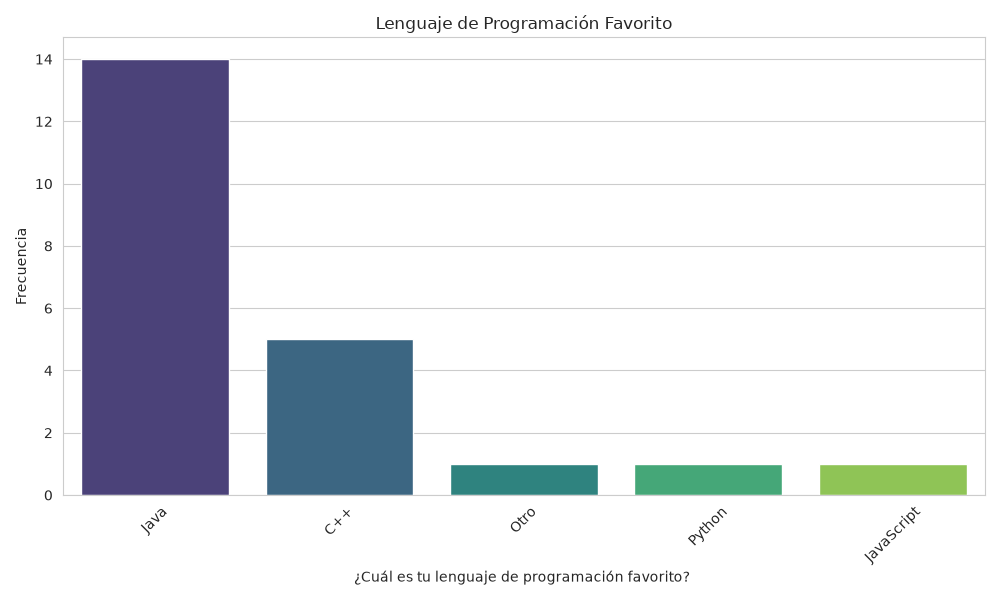
\includegraphics[width=0.9\textwidth]{Figure2barras.png}
    \caption{Distribución de lenguajes de programación favoritos — diagrama de barras}
    \label{fig:barras-lenguajes}
\end{figure}

\begin{figure}[H]
    \centering
    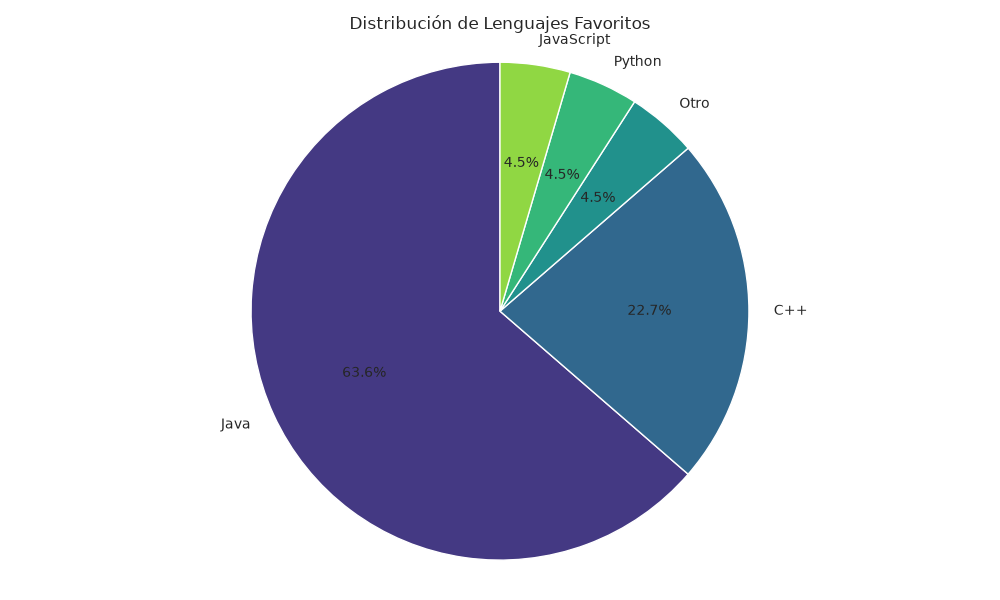
\includegraphics[width=0.8\textwidth]{FigureCircular.png}
    \caption{Distribución de lenguajes de programación favoritos — diagrama circular}
    \label{fig:circular-lenguajes}
\end{figure}

\newpage
% =========================================================
% ========== SEGUNDA VARIABLE: HORAS PROGRAMANDO ==========
% =========================================================

% =========================================================
% ================ FICHA TÉCNICA DE LA VARIABLE ==========
% =========================================================
\section*{Ficha técnica}

\begin{tabularx}{\textwidth}{@{}l X@{}}
\textbf{Variable estadística $X$:} & Cantidad de horas programando (horas enteras) \\[4pt]
\textbf{Población:} & Estudiantes de 2do año de Ingeniería de Sistemas \\[4pt]
\textbf{Muestra:} & 22 estudiantes de EMAT, grupo B \\[4pt]
\textbf{Unidad de observación:} & Un estudiante individual \\[4pt]
\textbf{Fuente:} & Recolección de datos mediante formulario de Google Forms \\[4pt]
\textbf{Tipo de dato estadístico:} & Cuantitativo discreto \\
\end{tabularx}

\vspace{1cm}

% =========================================================
% ============ TABLA DE DISTRIBUCIÓN DE FRECUENCIAS ======
% =========================================================
\section*{Tabla de distribución de frecuencias}

\begin{table}[H]
    \centering
    \caption{Cantidad de horas programando de los estudiantes de EMAT B(horas enteras)}
    \label{tab:horas-programando}
    \begin{tabular}{@{}cccccc@{}}
        \toprule
        $x_i$ & $f_i$ & $F_i$ & $h_i$ & $H_i$ & $h_i\%$ \\
        \midrule
        2 & 4 & 4 & 0.1818 & 0.1818 & 18.18\% \\
        5 & 4 & 8 & 0.1818 & 0.3636 & 18.18\% \\
        10 & 4 & 12 & 0.1818 & 0.5455 & 18.18\% \\
        15 & 3 & 15 & 0.1364 & 0.6818 & 13.64\% \\
        22 & 3 & 18 & 0.1364 & 0.8182 & 13.64\% \\
        28 & 1 & 19 & 0.0455 & 0.8636 & 4.55\% \\
        30 & 1 & 20 & 0.0455 & 0.9091 & 4.55\% \\
        40+ & 2 & 22 & 0.0909 & 1.0000 & 9.09\% \\
        \midrule
        \textbf{Total} & 22 & & 1.0000 & & 100\% \\
        \bottomrule
    \end{tabular}
\end{table}

\noindent\textbf{Notación utilizada:}
\begin{itemize}[leftmargin=2cm]
    \item[$x_i$] Valor de la variable (horas programando)
    \item[$f_i$] Frecuencia absoluta
    \item[$F_i$] Frecuencia absoluta acumulada
    \item[$h_i$] Frecuencia relativa
    \item[$H_i$] Frecuencia relativa acumulada
    \item[$h_i\%$] Porcentaje
\end{itemize}

% =========================================================
% ==================== DIAGRAMAS ==========================
% =========================================================
\section*{Representación gráfica}

\begin{figure}[H]
    \centering
    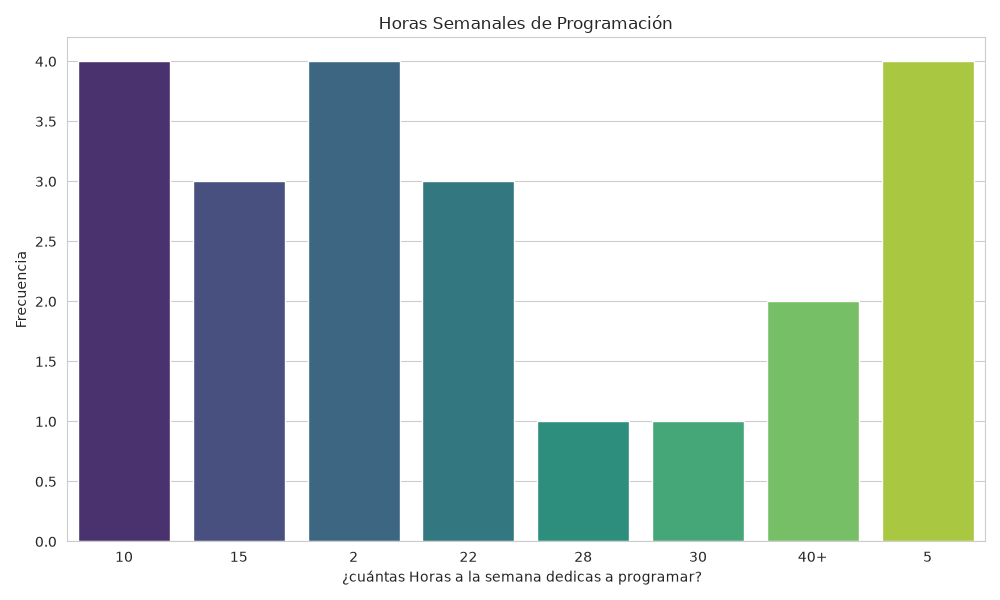
\includegraphics[width=0.9\textwidth]{FigureBarras1png.png}
    \caption{Distribución de horas programando — gráfico de barras}
    \label{fig:barras-horas}
\end{figure}

\begin{figure}[H]
    \centering
    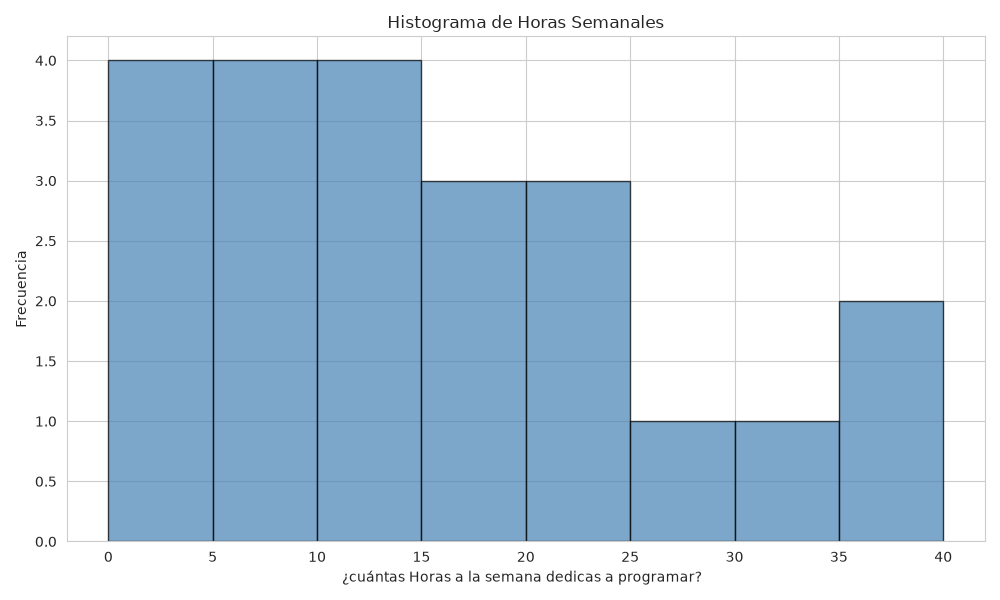
\includegraphics[width=0.8\textwidth]{FigureHistograma1.png}
    \caption{Distribución de horas programando — histograma}
    \label{fig:histograma-horas}
\end{figure}

\section*{Medidas de tendencia central}

\subsection*{1. Promedio (Media Aritmética)}
\begin{equation*}
    \bar{x} = \frac{\sum_{i=1}^{k} x_i \cdot f_i}{n}
\end{equation*}

\textbf{Notación:}
\begin{itemize}
    \item $x_i$: valor de la variable
    \item $f_i$: frecuencia absoluta de $x_i$
    \item $n$: tamaño de la muestra
\end{itemize}

\begin{table}[H]
    \centering
    \caption{Cantidad de horas programando de los estudiantes de EMAT B(horas enteras)}
    \label{tab:media-horas-programando}
    \begin{tabular}{@{}lccc@{}}
        \toprule
        $x_i$ & $f_i$ & $x_i \cdot f_i$ \\
        \midrule
        2 & 4 & 8 \\
        5 & 4 & 20 \\
        10 & 4 & 40 \\
        15 & 3 & 45 \\
        22 & 3 & 66 \\
        28 & 1 & 28 \\
        30 & 1 & 30 \\
        40+ & 2 & 80 \\
        \midrule
        \textbf{Total} & \textbf{22} & \textbf{317} \\
        \bottomrule
    \end{tabular}
\end{table}

\textbf{Desarrollo:}
\begin{equation*}
    \bar{x} = \frac{317}{22} \approx 14.41
\end{equation*}

\textbf{Interpretación:} Los estudiantes de EMAT B dedican en promedio 14 horas programando a la semana.

\subsection*{2. Mediana (Md)}
\begin{equation*}
    \text{Posición} = \frac{n}{2}
\end{equation*}

\textbf{Notación:}
\begin{itemize}
    \item $n$: tamaño de la muestra (total de elementos)
\end{itemize}

\begin{table}[H]
    \centering
    \caption{Cantidad de horas programando de los estudiantes de EMAT B(horas enteras)}
    \label{tab:mediana-cuantiles-horas}
    \begin{tabular}{@{}ccc@{}}
        \toprule
        $x_i$ & $f_i$ & $F_i$ \\
        \midrule
        2 & 4 & 4 \\
        5 & 4 & 8 \\
        10 & 4 & 12 \\
        15 & 3 & 15 \\
        22 & 3 & 18 \\
        28 & 1 & 19 \\
        30 & 1 & 20 \\
        40+ & 2 & 22 \\
        \midrule
        \textbf{Total} & \textbf{22} & \\
        \bottomrule
    \end{tabular}
\end{table}

\textbf{Desarrollo:}

\begin{itemize}
    \item Posición $= \dfrac{22}{2} = 11$
    \item Como $n$ es par, se promedian los valores en las posiciones 11 y 12.
    \item Buscando en $F_i$: ambas posiciones caen dentro de $F_i = 12$ (correspondiente a $x_i = 10$).
\end{itemize}
\begin{equation*}
    Md = \frac{10 + 10}{2} = 10
\end{equation*}

\textbf{Interpretación:} El 50\% de los estudiantes de EMAT B dedica a lo mucho 10 horas programando a la semana, mientras que el otro 50% dedica 10 horas o más.

\subsection*{3. Moda (Mo)}
\begin{equation*}
    Mo = x_i \text{ tal que } f_i \text{ es máxima}
\end{equation*}

\textbf{Notación:}
\begin{itemize}
    \item $x_i$: valor de la variable
    \item $f_i$: frecuencia absoluta de $x_i$
\end{itemize}

\begin{table}[H]
    \centering
    \caption{Cantidad de horas programando de los estudiantes de EMAT B(horas enteras)}
    \label{tab:moda-horas}
    \begin{tabular}{@{}cc@{}}
        \toprule
        $x_i$ & $f_i$ \\
        \midrule
        2 & 4 \\
        5 & 4 \\
        10 & 4 \\
        15 & 3 \\
        22 & 3 \\
        28 & 1 \\
        30 & 1 \\
        40+ & 2 \\
        \midrule
        \textbf{Total} & \textbf{22} \\
        \bottomrule
    \end{tabular}
\end{table}

\textbf{Desarrollo:}

La frecuencia máxima es $f_i = 4$, alcanzada por tres valores: $x_i = 2$, $x_i = 5$ y $x_i = 10$.
\begin{equation*}
    Mo = \{2,\ 5,\ 10\} \quad \text{(distribución trimodal)}
\end{equation*}

\textbf{Interpretación:} Los valores de horas que más se repiten entre los estudiantes de EMAT B son 2, 5 y 10 horas programando a la semana.

\subsection*{4. Cuartiles}
\begin{equation*}
    Q_j = L_i + a \cdot \frac{\left(\dfrac{j \cdot m}{4}\right) - F_{i-1}}{f_i}
\end{equation*}

\textbf{Notación:}
\begin{itemize}
    \item $L_i$: valor $x_i$ de la fila donde se ubica la posición (al ser datos no agrupados, $L_i = x_i$)
    \item $a$: amplitud de clase; para datos no agrupados $a = 0$
    \item $m$: tamaño de la muestra ($m=22$)
    \item $j$: número del cuartil a calcular ($j=1,2,3$)
    \item $F_{i-1}$: frecuencia acumulada de la fila anterior
    \item $f_i$: frecuencia absoluta de la fila donde se ubica la posición
\end{itemize}

\begin{table}[H]
    \centering
    \caption{Cantidad de horas programando de los estudiantes de EMAT B(horas enteras)}
    \label{tab:mediana-cuantiles-horas}
    \begin{tabular}{@{}ccc@{}}
        \toprule
        $x_i$ & $f_i$ & $F_i$ \\
        \midrule
        2 & 4 & 4 \\
        5 & 4 & 8 \\
        10 & 4 & 12 \\
        15 & 3 & 15 \\
        22 & 3 & 18 \\
        28 & 1 & 19 \\
        30 & 1 & 20 \\
        40+ & 2 & 22 \\
        \midrule
        \textbf{Total} & \textbf{22} & \\
        \bottomrule
    \end{tabular}
\end{table}

\textbf{Desarrollo:}

\begin{itemize}
    \item $Q_1$: $\dfrac{(1)(22)}{4}=5.5 \Rightarrow$ cae en $F_i=8$ ($x_i=5$)
    \begin{equation*}
        Q_1 = 5 + 0 \cdot \frac{5.5 - 4}{4} = 5
    \end{equation*}
    \item $Q_2$: $\dfrac{(2)(22)}{4}=11 \Rightarrow$ cae en $F_i=12$ ($x_i=10$)
    \begin{equation*}
        Q_2 = 10 + 0 \cdot \frac{11 - 8}{4} = 10
    \end{equation*}
    \item $Q_3$: $\dfrac{(3)(22)}{4}=16.5 \Rightarrow$ cae en $F_i=18$ ($x_i=22$)
    \begin{equation*}
        Q_3 = 22 + 0 \cdot \frac{16.5 - 15}{3} = 22
    \end{equation*}
\end{itemize}

\textbf{Interpretación:} Por ejemplo para $Q_1$, el 25\% de los estudiantes de EMAT B dedica a lo mucho 5 horas programando a la semana, mientras que el otro 75\% dedica 5 horas o más.

\subsection*{5. Deciles}
\begin{equation*}
    D_j = L_i + a \cdot \frac{\left(\dfrac{j \cdot m}{10}\right) - F_{i-1}}{f_i}
\end{equation*}

\textbf{Notación:}
\begin{itemize}
    \item $L_i$: valor $x_i$ de la fila donde se ubica la posición ($L_i = x_i$ por ser datos no agrupados)
    \item $a$: amplitud de clase; $a = 0$
    \item $m$: tamaño de la muestra ($m=22$)
    \item $j$: número del decil a calcular ($j=1,2,\dots,9$)
    \item $F_{i-1}$: frecuencia acumulada de la fila anterior
    \item $f_i$: frecuencia absoluta de la fila donde se ubica la posición
\end{itemize}

\begin{table}[H]
    \centering
    \caption{Cantidad de horas programando de los estudiantes de EMAT B(horas enteras)}
    \label{tab:mediana-cuantiles-horas}
    \begin{tabular}{@{}ccc@{}}
        \toprule
        $x_i$ & $f_i$ & $F_i$ \\
        \midrule
        2 & 4 & 4 \\
        5 & 4 & 8 \\
        10 & 4 & 12 \\
        15 & 3 & 15 \\
        22 & 3 & 18 \\
        28 & 1 & 19 \\
        30 & 1 & 20 \\
        40+ & 2 & 22 \\
        \midrule
        \textbf{Total} & \textbf{22} & \\
        \bottomrule
    \end{tabular}
\end{table}

\textbf{Desarrollo:}

\begin{itemize}
    \item $D_1$: $2.2 \Rightarrow F_i=4$ ($x_i=2$) $\Rightarrow D_1 = 2 + 0\cdot\frac{2.2-0}{4} = 2$
    \item $D_2$: $4.4 \Rightarrow F_i=8$ ($x_i=5$) $\Rightarrow D_2 = 5 + 0\cdot\frac{4.4-4}{4} = 5$
    \item $D_3$: $6.6 \Rightarrow F_i=8$ ($x_i=5$) $\Rightarrow D_3 = 5 + 0\cdot\frac{6.6-4}{4} = 5$
    \item $D_4$: $8.8 \Rightarrow F_i=12$ ($x_i=10$) $\Rightarrow D_4 = 10 + 0\cdot\frac{8.8-8}{4} = 10$
    \item $D_5$: $11 \Rightarrow F_i=12$ ($x_i=10$) $\Rightarrow D_5 = 10 + 0\cdot\frac{11-8}{4} = 10$
    \item $D_6$: $13.2 \Rightarrow F_i=15$ ($x_i=15$) $\Rightarrow D_6 = 15 + 0\cdot\frac{13.2-12}{3} = 15$
    \item $D_7$: $15.4 \Rightarrow F_i=18$ ($x_i=22$) $\Rightarrow D_7 = 22 + 0\cdot\frac{15.4-15}{3} = 22$
    \item $D_8$: $17.6 \Rightarrow F_i=18$ ($x_i=22$) $\Rightarrow D_8 = 22 + 0\cdot\frac{17.6-15}{3} = 22$
    \item $D_9$: $19.8 \Rightarrow F_i=20$ ($x_i=30$) $\Rightarrow D_9 = 30 + 0\cdot\frac{19.8-19}{1} = 30$
\end{itemize}

\textbf{Interpretación:} Para $D_1$, el 10\% de los estudiantes de EMAT B dedica a lo mucho 2 horas programando a la semana.

\subsection*{6. Percentiles}
\begin{equation*}
    P_j = L_i + a \cdot \frac{\left(\dfrac{j \cdot m}{100}\right) - F_{i-1}}{f_i}
\end{equation*}

\textbf{Notación:}
\begin{itemize}
    \item $L_i$: valor $x_i$ de la fila donde se ubica la posición ($L_i = x_i$ por ser datos no agrupados)
    \item $a$: amplitud de clase; $a = 0$
    \item $m$: tamaño de la muestra ($m=22$)
    \item $j$: número del percentil a calcular ($j=1,2,\dots,99$)
    \item $F_{i-1}$: frecuencia acumulada de la fila anterior
    \item $f_i$: frecuencia absoluta de la fila donde se ubica la posición
\end{itemize}

\begin{table}[H]
    \centering
    \caption{Cantidad de horas programando de los estudiantes de EMAT B(horas enteras)}
    \label{tab:mediana-cuantiles-horas}
    \begin{tabular}{@{}ccc@{}}
        \toprule
        $x_i$ & $f_i$ & $F_i$ \\
        \midrule
        2 & 4 & 4 \\
        5 & 4 & 8 \\
        10 & 4 & 12 \\
        15 & 3 & 15 \\
        22 & 3 & 18 \\
        28 & 1 & 19 \\
        30 & 1 & 20 \\
        40+ & 2 & 22 \\
        \midrule
        \textbf{Total} & \textbf{22} & \\
        \bottomrule
    \end{tabular}
\end{table}

\textbf{Desarrollo:}

Se muestran los percentiles más usados como ejemplo:
\begin{itemize}
    \item $P_{10}$: $2.2 \Rightarrow F_i=4$ ($x_i=2$) $\Rightarrow P_{10} = 2 + 0\cdot\frac{2.2-0}{4} = 2$
    \item $P_{25}$: $5.5 \Rightarrow F_i=8$ ($x_i=5$) $\Rightarrow P_{25} = 5 + 0\cdot\frac{5.5-4}{4} = 5$ \quad ($=Q_1$)
    \item $P_{50}$: $11 \Rightarrow F_i=12$ ($x_i=10$) $\Rightarrow P_{50} = 10 + 0\cdot\frac{11-8}{4} = 10$ \quad ($=Md=Q_2$)
    \item $P_{75}$: $16.5 \Rightarrow F_i=18$ ($x_i=22$) $\Rightarrow P_{75} = 22 + 0\cdot\frac{16.5-15}{3} = 22$ \quad ($=Q_3$)
    \item $P_{90}$: $19.8 \Rightarrow F_i=20$ ($x_i=30$) $\Rightarrow P_{90} = 30 + 0\cdot\frac{19.8-19}{1} = 30$
\end{itemize}

\textbf{Interpretación:} Para $P_{10}$, el 10\% de los estudiantes de EMAT B dedica a lo mucho 2 horas programando a la semana.
\end{document}